
%(BEGIN_QUESTION)
% Copyright 2006, Tony R. Kuphaldt, released under the Creative Commons Attribution License (v 1.0)
% This means you may do almost anything with this work of mine, so long as you give me proper credit

Pictured here is a P\&ID (Process and Instrument Diagram) of a liquid flow control ``loop,'' consisting of a {\it flow transmitter} (FT) to sense liquid flow rate through the pipe and output an electronic signal corresponding to the flow, a {\it flow controller} (FC) to sense the flow signal and decide which way the control valve should move, a current-to-air (I/P) {\it transducer} (FY) to convert the controller's electronic output signal into a variable air pressure, and an air-operated {\it flow control valve} (FV) to throttle the liquid flow:

$$\includegraphics[width=15.5cm]{i00124x01.eps}$$

The actions of each instrument are shown here:

\begin{itemize}
\item{} FT: increasing liquid flow = increasing current signal
\item{} FC: increasing process variable (input) signal = decreasing output signal
\item{} FY: increasing current input signal = increasing pneumatic output signal
\item{} FV: increasing pneumatic signal = open more
\end{itemize}

Describe what will happen to all signals in this control loop with the controller in ``automatic'' mode (ready to compensate for any changes in flow rate by automatically moving the valve) if the pump were to suddenly spin faster and create more fluid pressure, causing an increase in flow rate.

Also describe what will happen to all signals in this control loop with the controller in ``manual'' mode (where the output signal remains set at whatever level the human operator sets it at) if the pump were to suddenly spin faster and create more fluid pressure, causing an increase in flow rate.

\vskip 20pt \vbox{\hrule \hbox{\strut \vrule{} {\bf Suggestions for Socratic discussion} \vrule} \hrule}

\begin{itemize}
\item{} Explain the practical benefit of having a ``manual'' mode in a process loop controller.  When might we intentionally use manual mode in an operating process condition?
\end{itemize}

\underbar{file i00124}
%(END_QUESTION)





%(BEGIN_ANSWER)

\noindent
{\bf In automatic mode:}

Process flow rate (increase) $\to$ FT output signal (increase milliamps) $\to$ FC output signal (decrease milliamps) $\to$ FY output signal (decrease PSI) $\to$ FV position (moves further closed, pinching off liquid flow).

\vskip 10pt

\noindent
{\bf In manual mode:}

Process flow rate (increase) $\to$ FT output signal (increase milliamps) $\to$ FC output signal (remains steady) $\to$ FY output signal (remains steady) $\to$ FV position (holds position).

\vskip 10pt

The important part of this question is the difference in response between ``automatic'' and ``manual'' controller modes.  In automatic control mode, the controller takes action to bring the process back to setpoint.  In manual control mode, the controller just lets the process drift and takes no action to stop it.

At first, having a ``manual'' mode in a control system seems pointless.  However, giving human operators the ability to manually override the otherwise automatic actions of a control system is important for start-up, shut-down, and handling emergency (unusual) conditions in a process system.  

Manual mode is also a very important diagnostic tool for instrument technicians and operators alike.  Being able to ``turn off the brain'' of an automatic control system and watch process response to manual changes in manipulated variable (final control element) signals gives technical personnel opportunity to test for unusual control valve behavior, process quirks, and other behaviors in a system that can lead to poor automatic control. 


%(END_ANSWER)





%(BEGIN_NOTES)




%INDEX% Control, basics: signal changes in an automatic control loop

%(END_NOTES)


